\begin{frame}[fragile]{Ramificación}
    \begin{columns}[T,onlytextwidth]
      \column{0.55\textwidth}
      \begin{itemize}
        \item \alert{Crear una rama}
          \mint{console}| $ git branch <nombre-rama>|
        \item \alert{Moverse entre ramas}
          \mint{console}| $ git checkout <nombre-rama>|
        \item \alert{Crear y moverse a la rama creada}
          \mint{console}| $ git checkout -b <nombre-rama>|
      \end{itemize}
      \column{0.45\textwidth}
        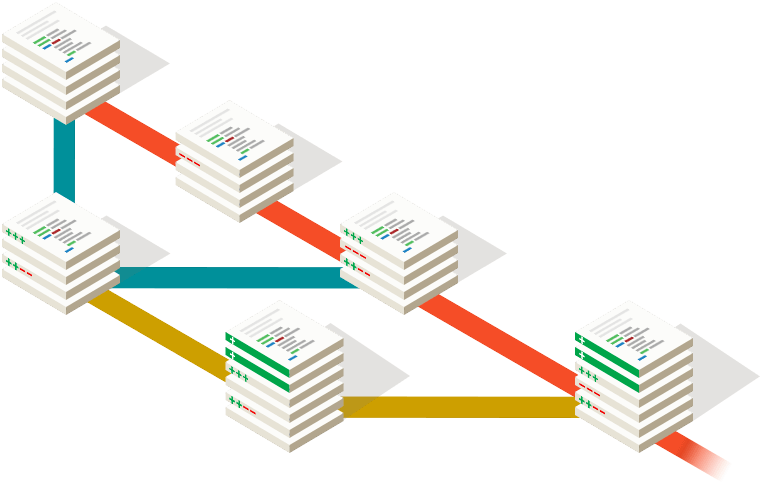
\includegraphics[scale=0.23]{images/branching-illustration}
    \end{columns}
\end{frame}

\begin{frame}[fragile]{Ramificación}
    \begin{columns}[T,onlytextwidth]
      \column{0.52\textwidth}
      \begin{exampleblock}{Ejemplo:}
        \uncover<2->{
        \mint{console}| $ git checkout -b issue53|}
        \uncover<3->{
        \mint{console}| $ git commit -am 'mensaje'|}
        \uncover<4->{
        \mint{console}| $ git checkout master|}
        \uncover<5->{
        \mint{console}| $ git checkout -b hotfix|}
        \uncover<6->{
        \mint{console}| $ git commit -am 'mensaje'|}
      \end{exampleblock}
      \column{0.48\textwidth}
        \begin{figure}
          \only<1>{\scalebox{.95}{\begin{tikzpicture}
  \gitDAG[grow right sep = 1.5em]{
    A -- B -- C
  };
  \gitbranch
    {master}      % node name and text
    {above=of C} % node placement
    {C}          % target
  % HDAD reference
  \gitHEAD
    {above=of master} % node placement
    {master}          % target
\end{tikzpicture}
}}
          \only<2>{\scalebox{.95}{\begin{tikzpicture}
  \gitDAG[grow right sep = 1.5em]{
    A -- B -- C
  };
  \gitbranch
    {master}      % node name and text
    {above=of C} % node placement
    {C}          % target
  \gitbranch
    {issue53}      % node name and text
    {below=of C} % node placement
    {C}          % target
  % HDAD reference
  \gitHEAD
    {below=of issue53} % node placement
    {issue53}          % target
\end{tikzpicture}
}}
          \only<3>{\scalebox{.95}{\begin{tikzpicture}
  \gitDAG[grow right sep = 1.5em]{
    A -- B -- C -- D
  };
  \gitbranch
    {master}      % node name and text
    {above=of C} % node placement
    {C}          % target
  \gitbranch
    {issue53}      % node name and text
    {below=of D} % node placement
    {D}          % target
  % HDAD reference
  \gitHEAD
    {below=of issue53} % node placement
    {issue53}          % target
\end{tikzpicture}
}}
          \only<4>{\scalebox{.95}{\begin{tikzpicture}
  \gitDAG[grow right sep = 1.5em]{
    A -- B -- C -- E
  };
  \gitbranch
    {master}      % node name and text
    {above=of C} % node placement
    {C}          % target
  \gitbranch
    {hotfix}      % node name and text
    {below=of E} % node placement
    {E}          % target
  % HDAD reference
  \gitHEAD
    {above=of master} % node placement
    {master}          % target
\end{tikzpicture}
}}
          \only<5>{\scalebox{.95}{\begin{tikzpicture}
  \gitDAG[grow right sep = 1.5em]{
    A -- B -- C -- {
    E,
    D},
  };
  \gitbranch
    {master}      % node name and text
    {above=of E} % node placement
    {E}          % target
  \gitbranch
    {issue53}      % node name and text
    {below=of D} % node placement
    {D}          % target
  % HDAD reference
  \gitHEAD
    {above=of master} % node placement
    {master}          % target
\end{tikzpicture}
}}
          \only<6>{\scalebox{.95}{\begin{tikzpicture}
  \gitDAG[grow right sep = 1.5em]{
    A -- B -- C -- {
    E,
    D},
  };
  \gitbranch
    {master}      % node name and text
    {above=of C} % node placement
    {C}          % target
  \gitbranch
    {issue53}      % node name and text
    {below=of D} % node placement
    {D}          % target
  \gitbranch
    {hotfix}      % node name and text
    {above=of E} % node placement
    {E}          % target
  % HDAD reference
  \gitHEAD
    {above=of hotfix} % node placement
    {hotfix}          % target
\end{tikzpicture}
}}
        \end{figure}
    \end{columns}
\end{frame}
